\documentclass{article}
\usepackage{fancyhdr}
\usepackage{setspace}
\usepackage{titlesec}
\usepackage{graphicx}
\usepackage{float}
\usepackage[style=apa, sorting=nyt]{biblatex}
\usepackage{geometry}
\usepackage{hyperref}

\geometry{a4paper, margin=1in}
% \addbibresource{references.bib}

\begin{document}

% ---------- Cover page ---64-------
\begin{titlepage}
\begin{center}
\vspace*{1cm}

Swinburne University of Technology \\
School of Science, Computing, and Emerging Technologies
\vspace{8cm}

SWE40006 - Software Deployment and Evolution \\
\textbf{Deployment Portfolio Task 2}
\vfill

Student name: Ngoc Van Nhi Do \\
Student ID: 105551765 \\
Submission date: [DO NOT FORGETTTTTTTTTTTTTTTTTTTTTTT]
\end{center}
\end{titlepage}

% ---------- Header + footer ----------
\pagestyle{fancy}
\fancyhead[L]{Ngoc Van Nhi Do}
\fancyhead[R]{105551765}
\fancyfoot{}
\renewcommand{\footrulewidth}{0.4pt}% default is 0pt
\fancyfoot[L]{SWE40006 - Software Deployment and Evolution (Semester 2 2026)}
\fancyfoot[R]{\small\thepage}

\newpage

\begin{center}
\vspace*{2px}
{\LARGE
\setlength{\baselineskip}{2em}
Deployment Portfolio Task 2
}
\end{center}

\section{Declared Target Level}

All four subtasks 2.1, 2.2, 2.3, and 2.4 were attempted.

Table~\ref{tab:links} below contain relevant links as proof of successful task execution.

\begin{table}[ht]
\centering
\caption{Publicly accessible URLs for live grading verification} 
\label{tab:links}
\vspace{2pt}
\def\arraystretch{1.5}
\begin{tabular}{|p{2cm}|p{14cm}|}
\hline
\textbf{Source} & \textbf{URL} \\
\hline
Task 2.1 & \url{https://swe40006-task-2-1-atbmg9a7daapdnec.australiaeast-01.azurewebsites.net} \\
\hline
Task 2.2 & \url{https://swe40006-task-2-2-f9emhph2gddzhker.australiaeast-01.azurewebsites.net/} \\
\hline
\end{tabular}
\end{table}

\section{Execution Evidence}

\subsection{Task 2.1}

For Task 2.1, I deployed a simple Node.js web application to Azure App Services, using Visual Studio Code and the Azure App Services extension.

First, I created the Node.js app consisting of the files \texttt{index.html}, \texttt{style.css}, \texttt{package.json} and \texttt{server.js}.

\begin{figure}[H]
\centering
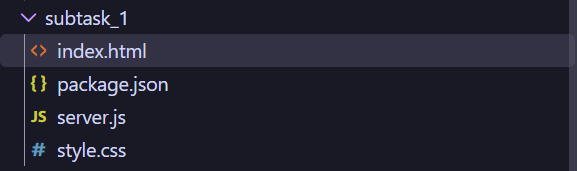
\includegraphics[scale=0.6]{images/1_node_app.jpg}
\vspace{-1em}
\caption{Structure of my simple Node.js application.}
\end{figure}

Then I ran my web application to test that it works correctly.

\begin{figure}[H]
\centering
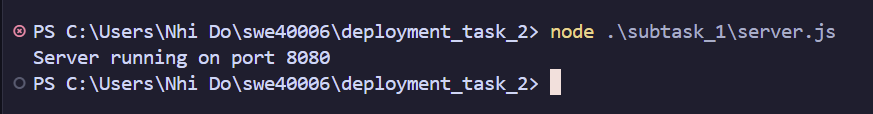
\includegraphics[scale=0.6]{images/1_test_npm.jpg}
\vspace{-1em}
\caption{Running \texttt{npm start} on my Node.js application.}
\end{figure}

\begin{figure}[H]
\centering
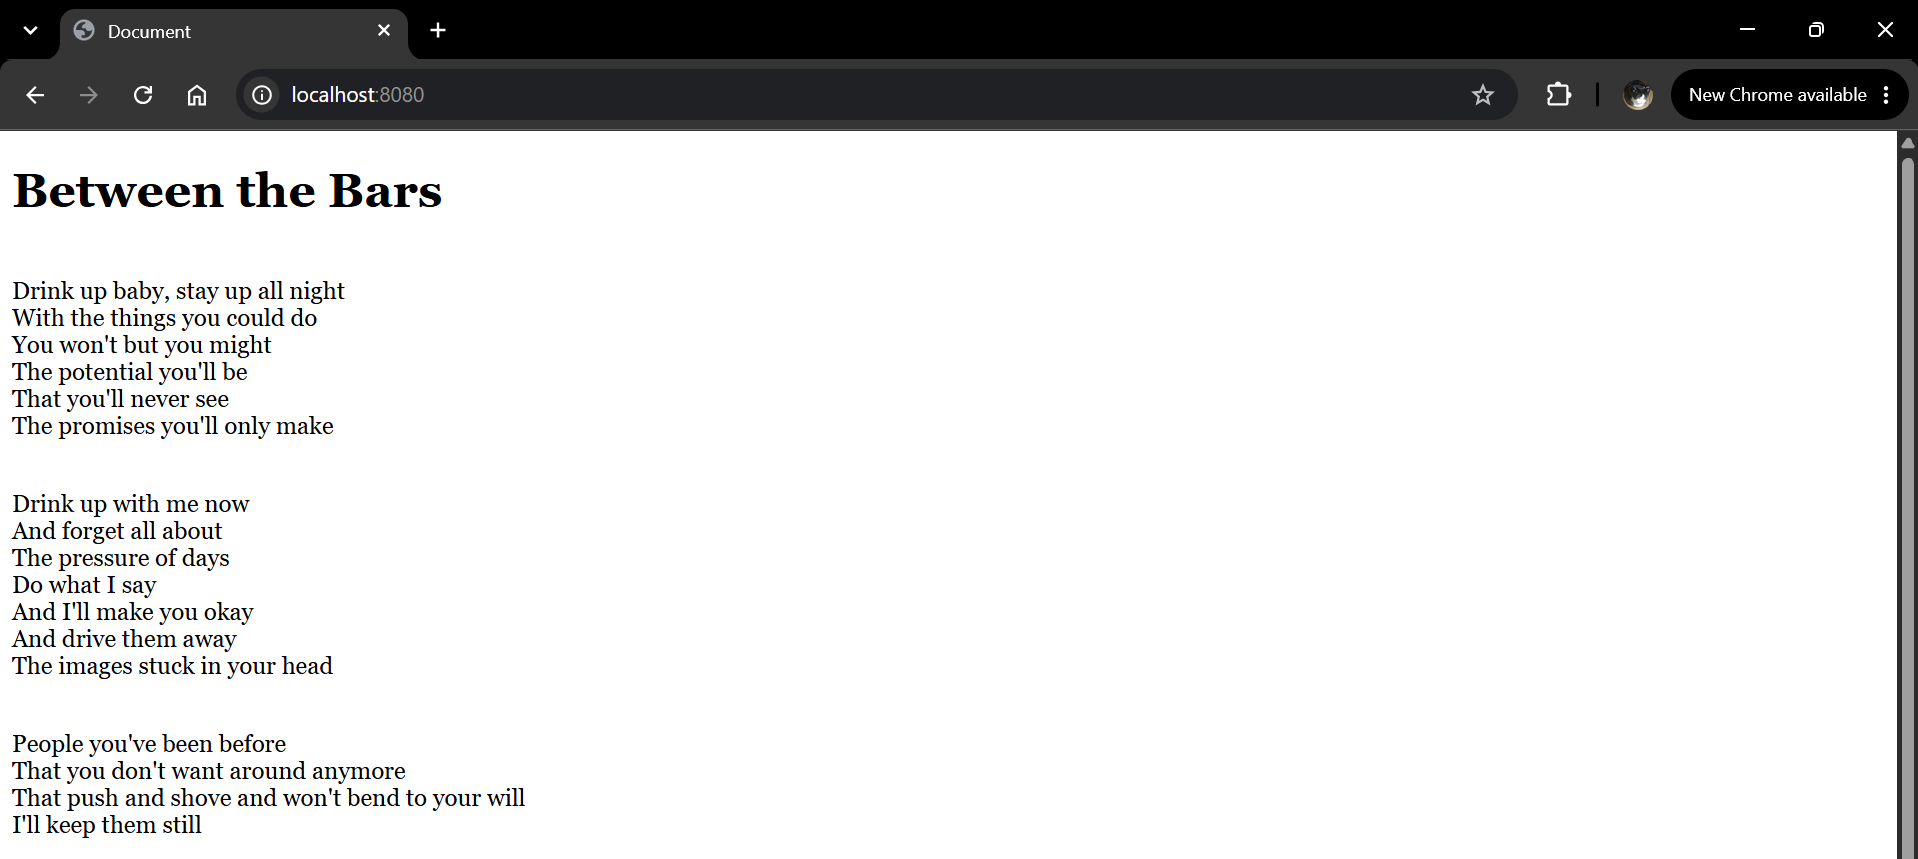
\includegraphics[scale=0.4]{images/1_test_app.jpg}
\vspace{-1em}
\caption{The web application runs locally on port 8080.}
\end{figure}

I then installed the Azure App Service on VS Code. The screenshot below shows the Azure panel once the extension has been successfully installed and I have logged in with my Azure account.

\begin{figure}[H]
\centering
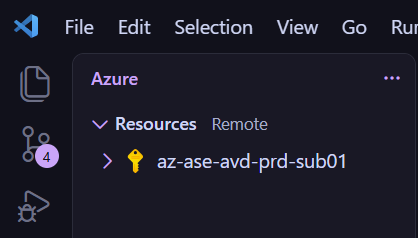
\includegraphics[scale=0.6]{images/1_azure_installed.jpg}
\vspace{-1em}
\caption{The Azure side panel on VS Code.}
\end{figure}

Next, I subscribed to an Azure for Students subscription on the Azure portal (\url{portal.azure.com}).

\begin{figure}[H]
\centering
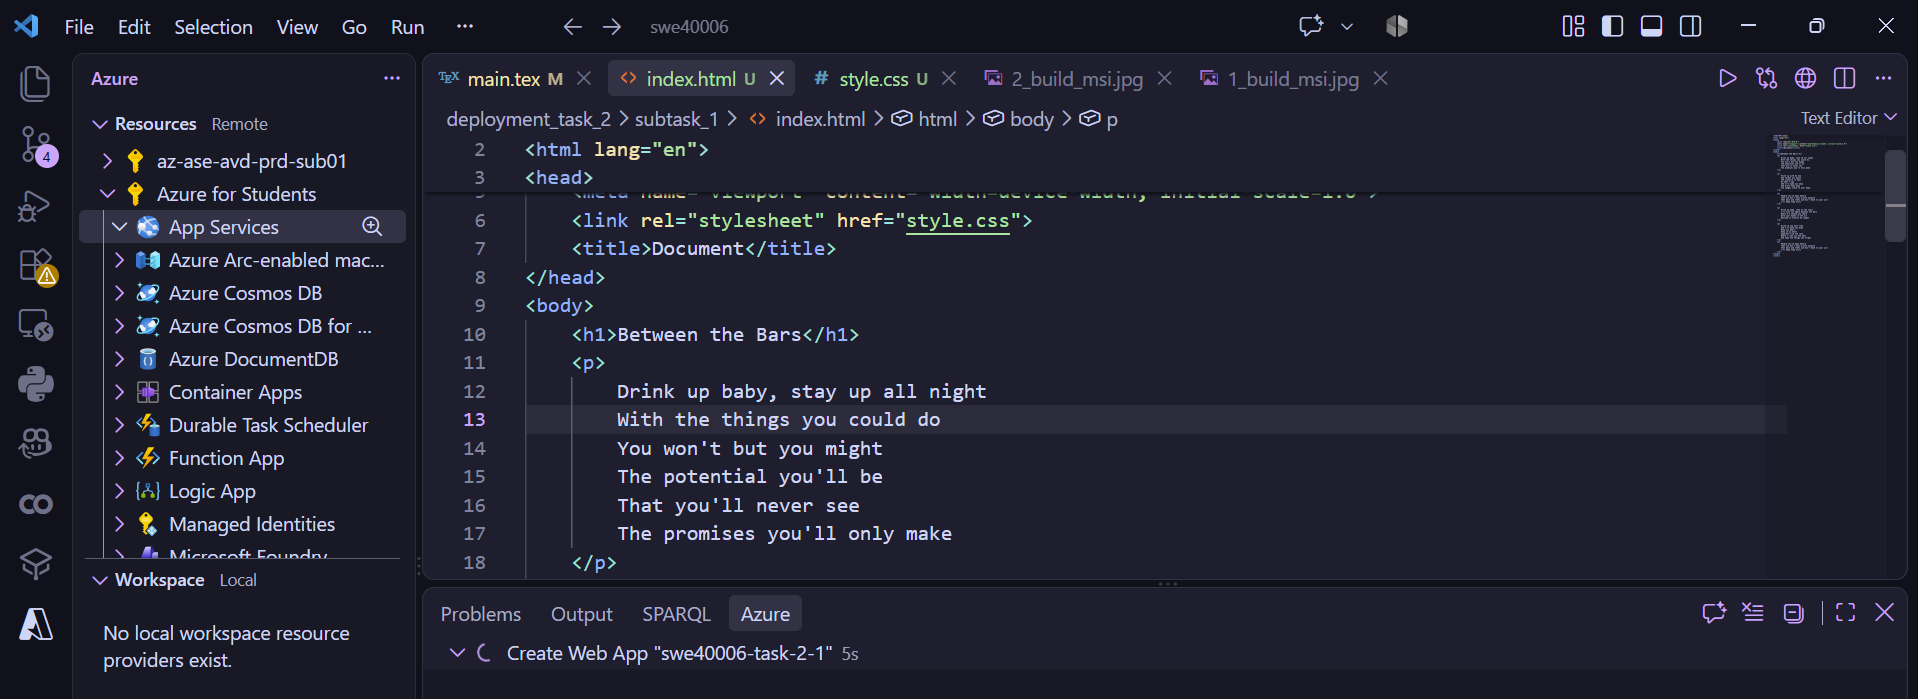
\includegraphics[scale=0.4]{images/1_azure_subscription.jpg}
\vspace{-1em}
\caption{The Azure panel updated with my new Azure for Students subscription.}
\end{figure}

I then created a new Azure Web App service using the "Create Web App" command. I specified the region where I wanted my web app to be hosted which was Australia East, the application name \texttt{swe40006-task-2-1}, and the technology stack which was Node LTS 24.

As seen below, initial attempts to create the web app failed as my subscription was not registered with the \texttt{Microsoft.OperationalInsights} namespace. This was resolved by registering with the namespace on the Azure Portal.

\begin{figure}[H]
\centering
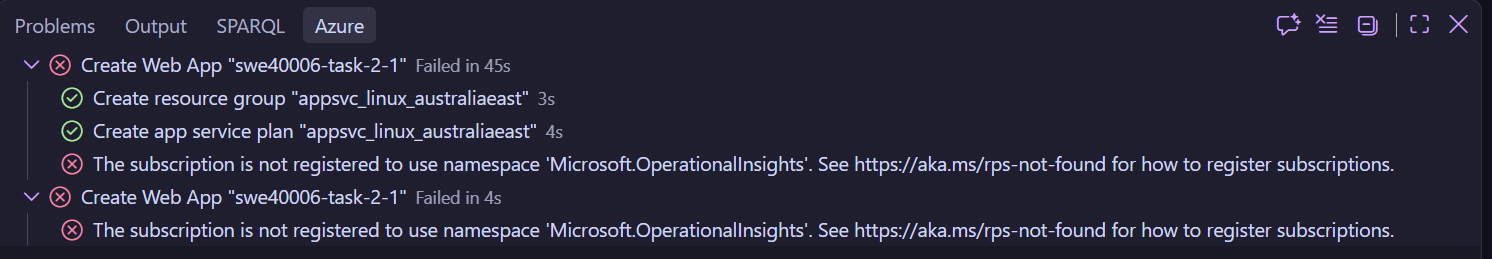
\includegraphics[scale=0.5]{images/1_unregistered_error.jpg}
\vspace{-1em}
\caption{Failed attempts at creating a new Azure App Service instance.}
\end{figure}

\begin{figure}[H]
\centering
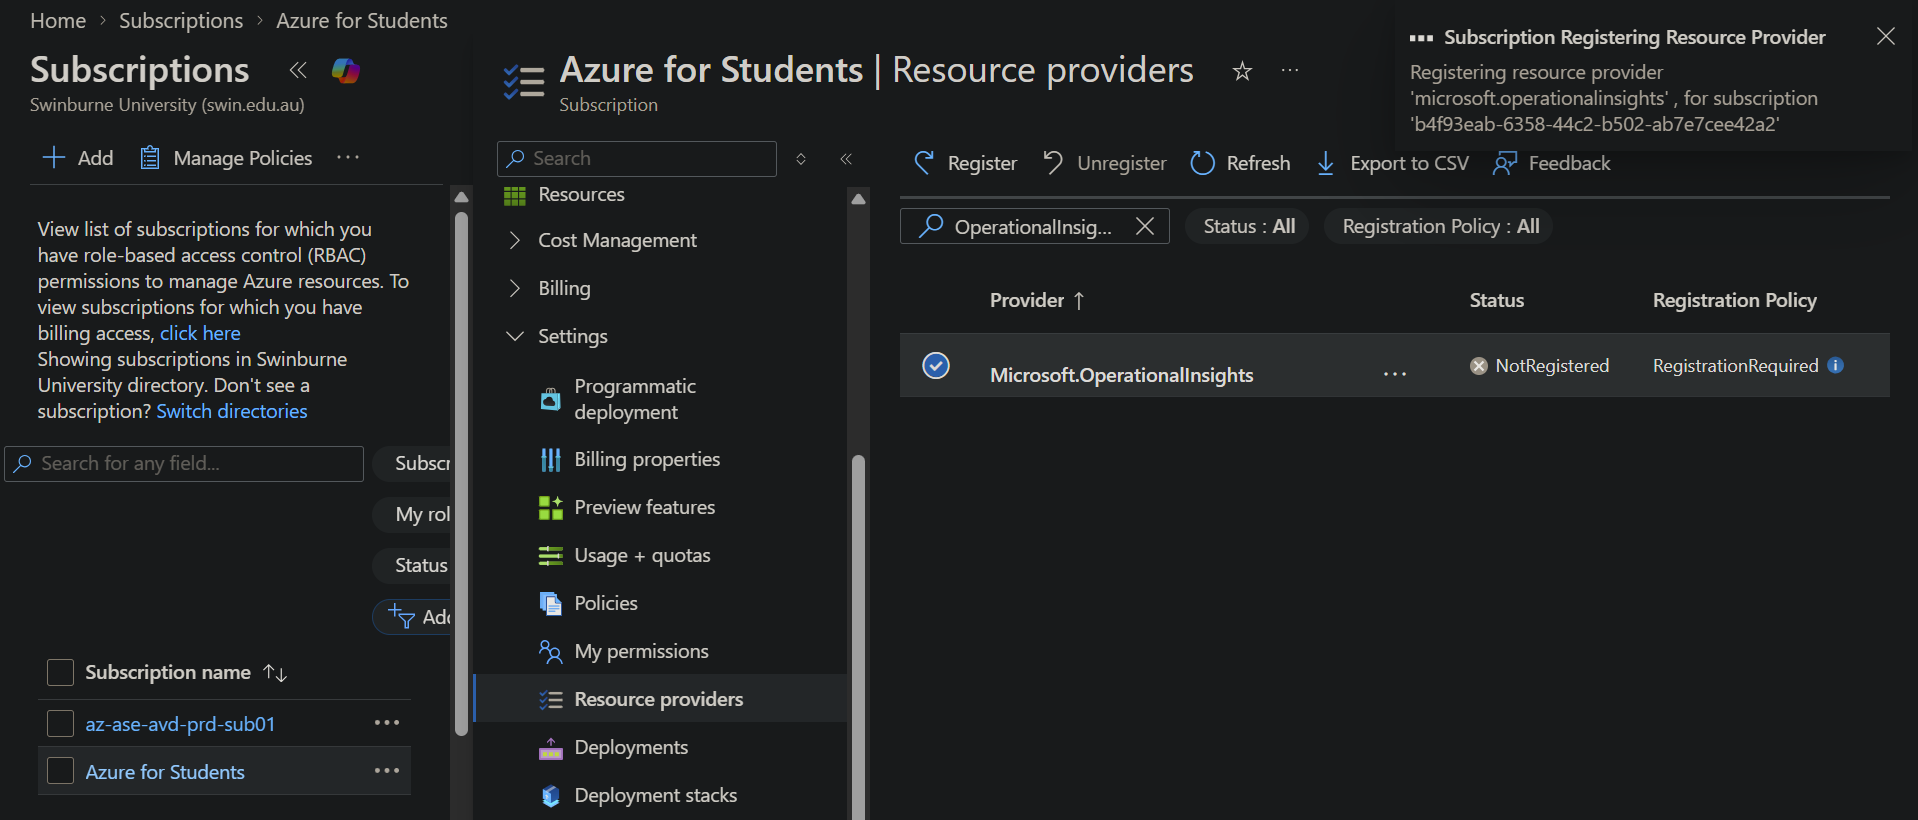
\includegraphics[scale=0.4]{images/1_register_namespace.jpg}
\vspace{-1em}
\caption{Registering with the \texttt{Microsoft.OperationalInsights} namespace on the Azure Portal.}
\end{figure}

\begin{figure}[H]
\centering
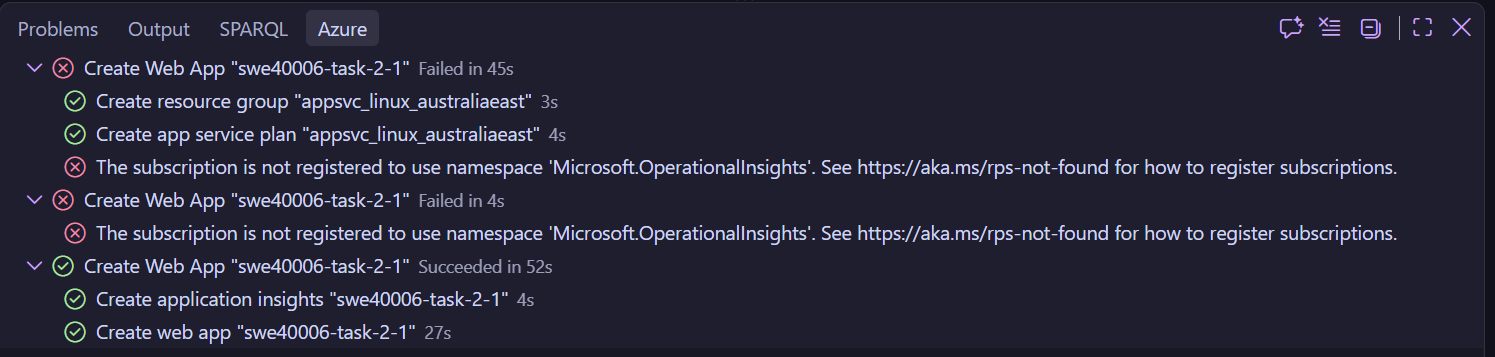
\includegraphics[scale=0.5]{images/1_create_web_app.jpg}
\vspace{-1em}
\caption{A new Azure App Service instance is successfully created.}
\end{figure}

The next step was to deploy my web application to the App Service instance. 

\begin{figure}[H]
\centering
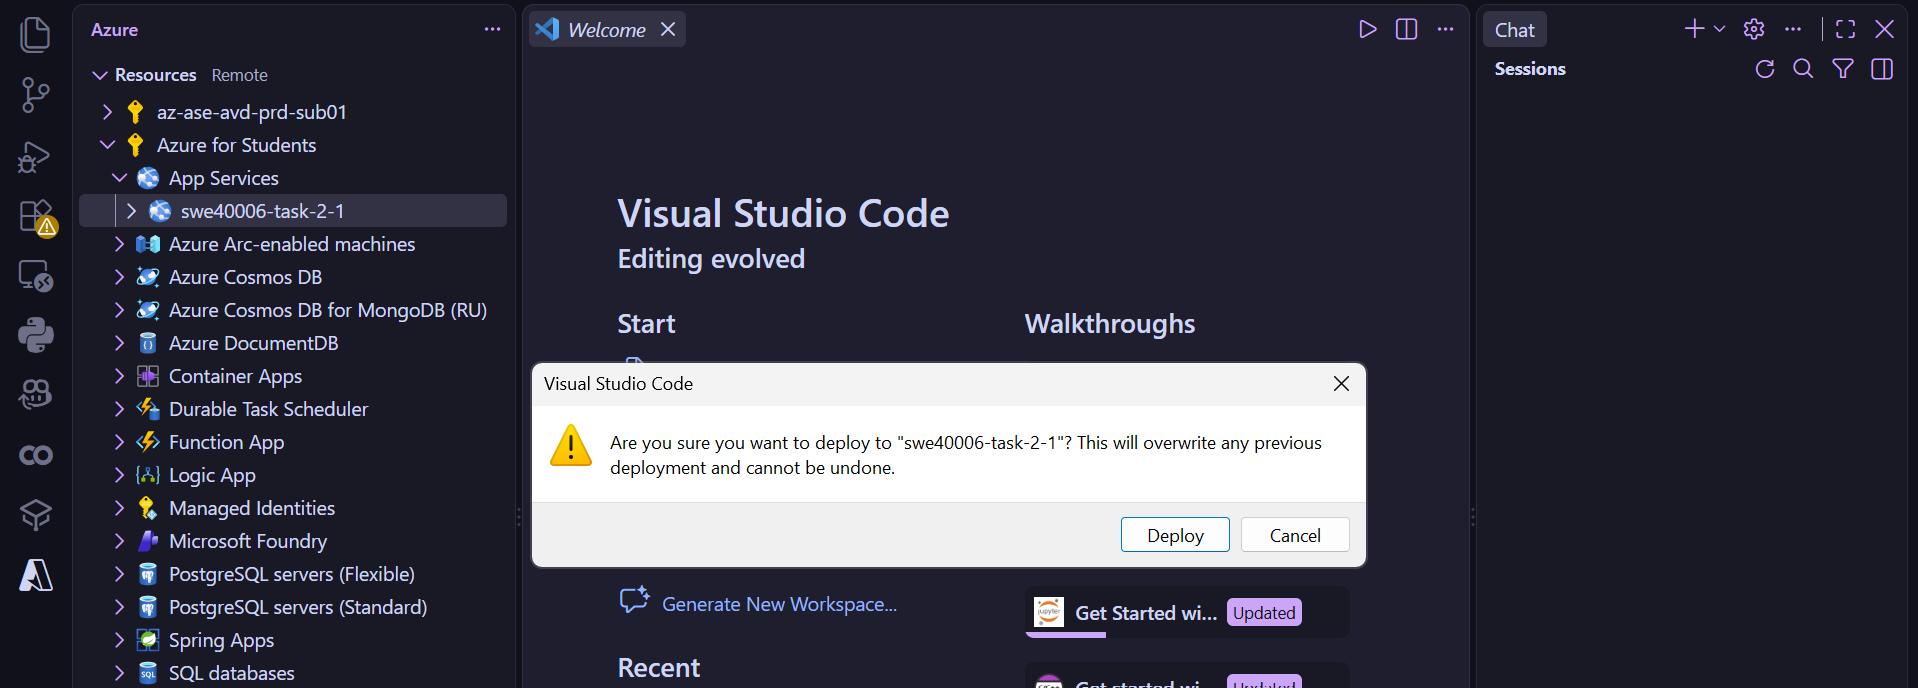
\includegraphics[scale=0.4]{images/1_deploy_web_app.jpg}
\vspace{-1em}
\caption{Deploying my web application to \texttt{swe40006-task-2-1}.}
\end{figure}

\begin{figure}[H]
\centering
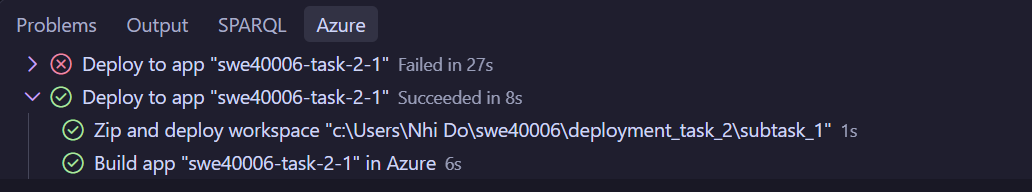
\includegraphics[scale=0.6]{images/1_deploy_success.jpg}
\vspace{-1em}
\caption{Deployment successful.}
\end{figure}

\begin{figure}[H]
\centering
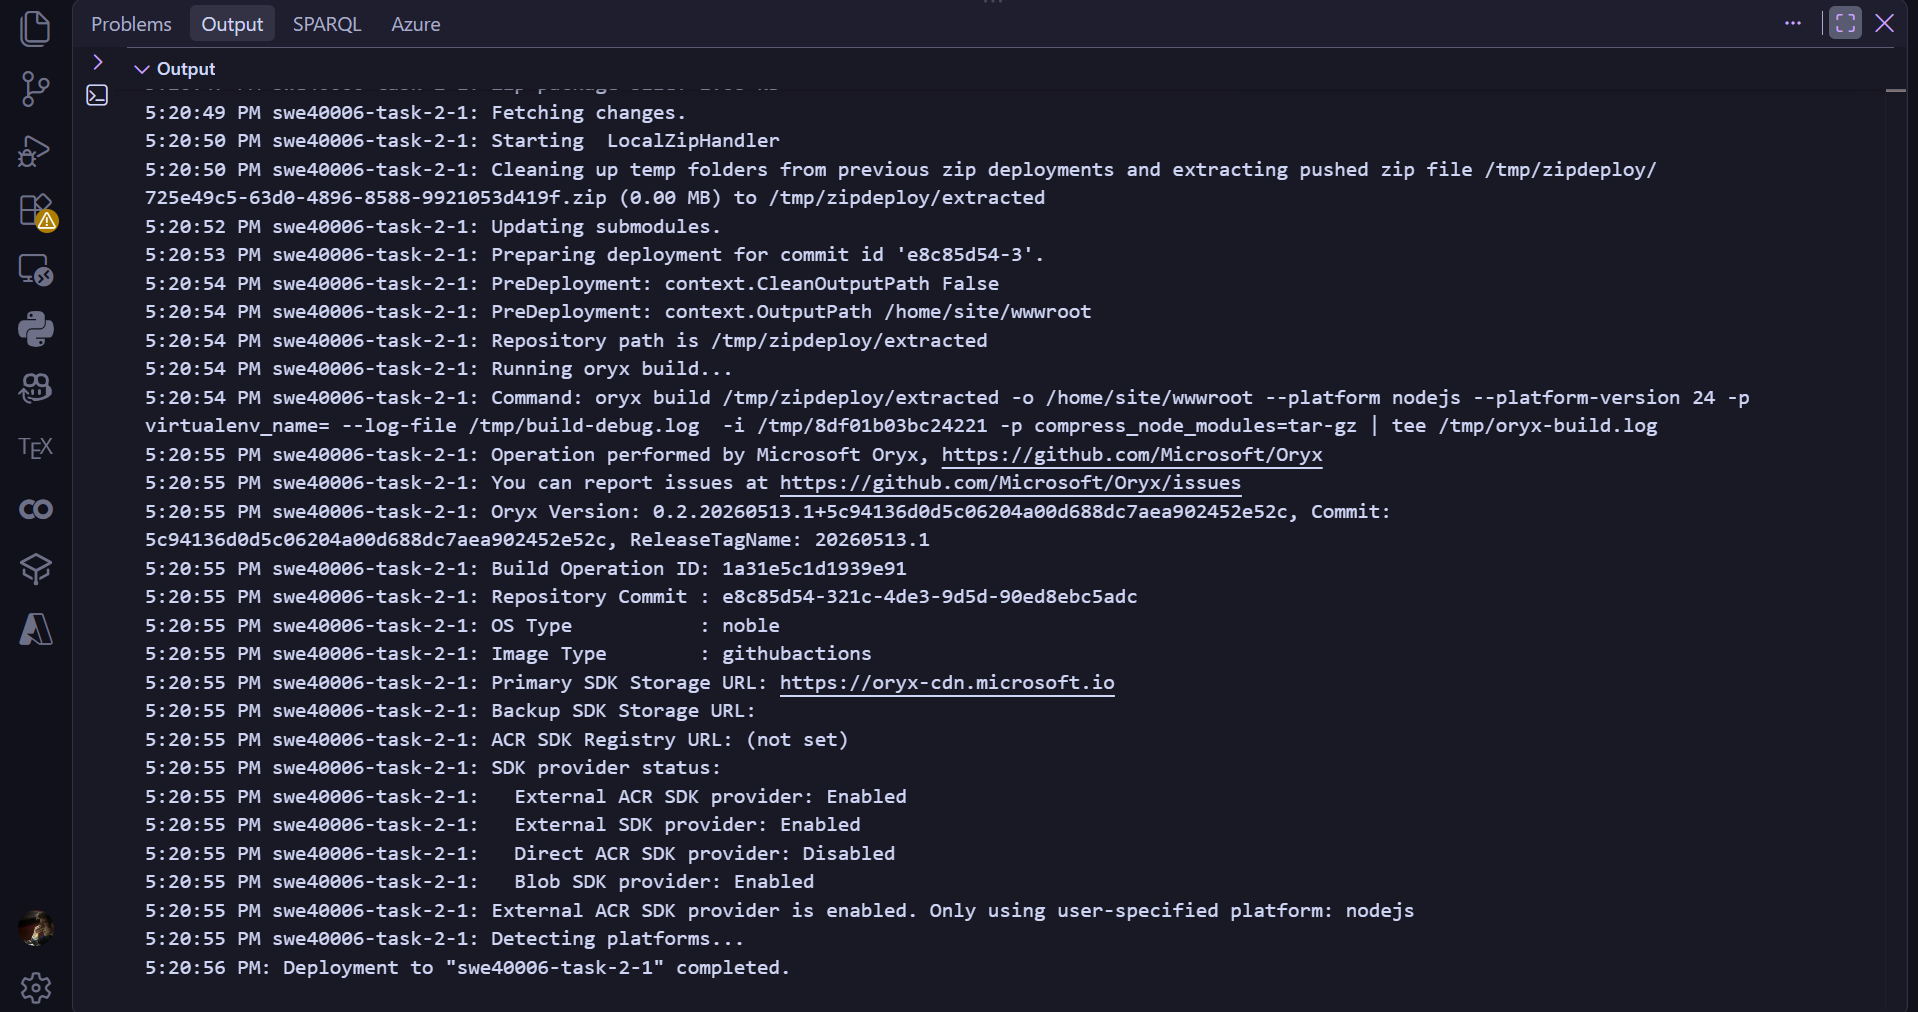
\includegraphics[scale=0.4]{images/1_build_output.jpg}
\vspace{-1em}
\caption{Build output.}
\end{figure}

The application is live and publicly acccessible at \url{https://swe40006-task-2-1-atbmg9a7daapdnec.australiaeast-01.azurewebsites.net}.

\begin{figure}[H]
\centering
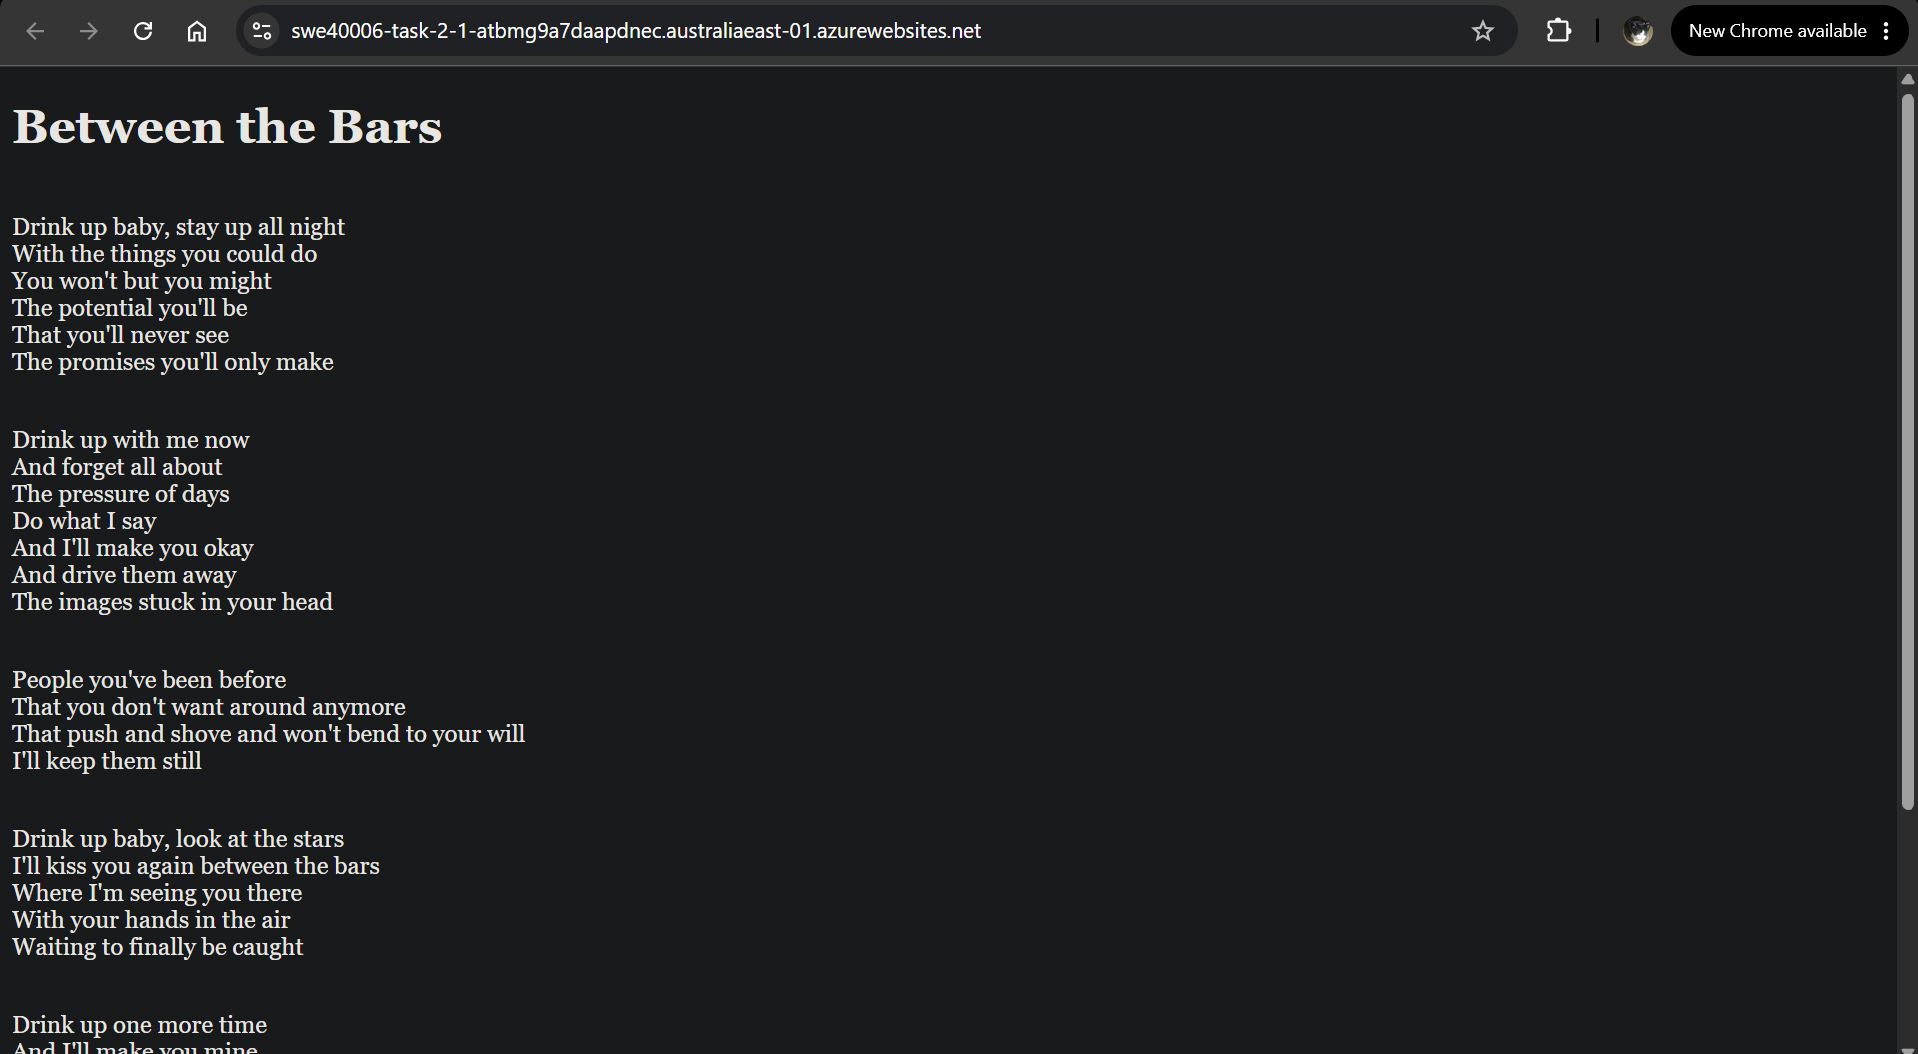
\includegraphics[scale=0.4]{images/1_live_site.jpg}
\vspace{-1em}
\caption{The application is deployed and running live.}
\end{figure}

\subsection{Task 2.2}

For task 2.2, I deployed an ASP.NET Razor Pages application with Azure App Services, also using Visual Studio Code and the Azure App Service extension.

First, I created a new Razor Pages project using the .NET CLI. Once the project has been created, I ran \texttt{dotnet publish} to publish the application.

\begin{figure}[H]
\centering
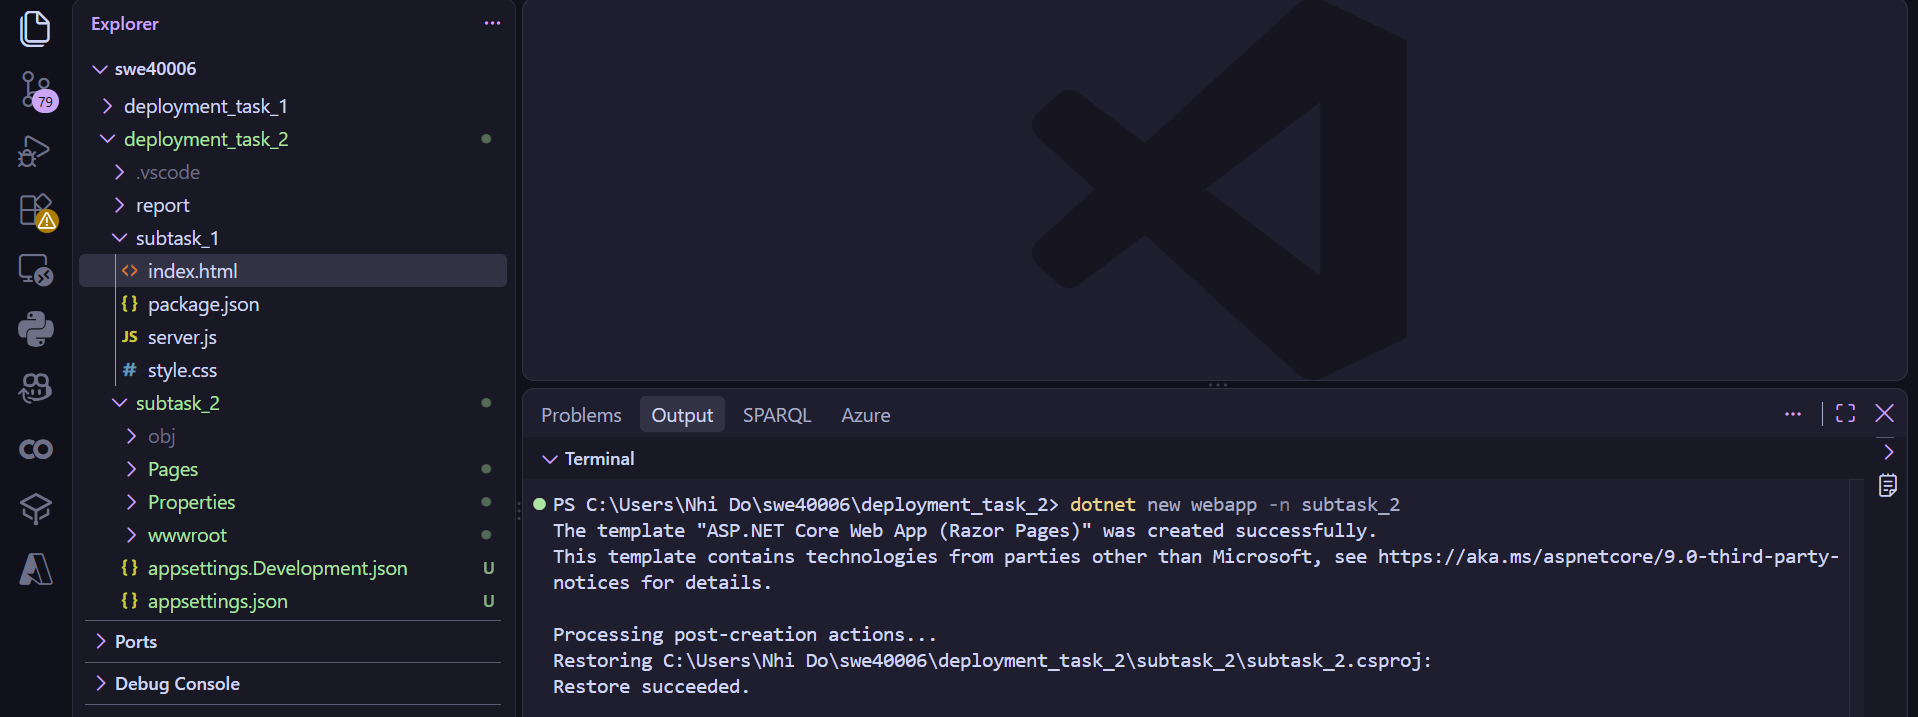
\includegraphics[scale=0.4]{images/2_new_project.jpg}
\vspace{-1em}
\caption{Creating a new Razor Pages project via the CLI.}
\end{figure}

\begin{figure}[H]
\centering
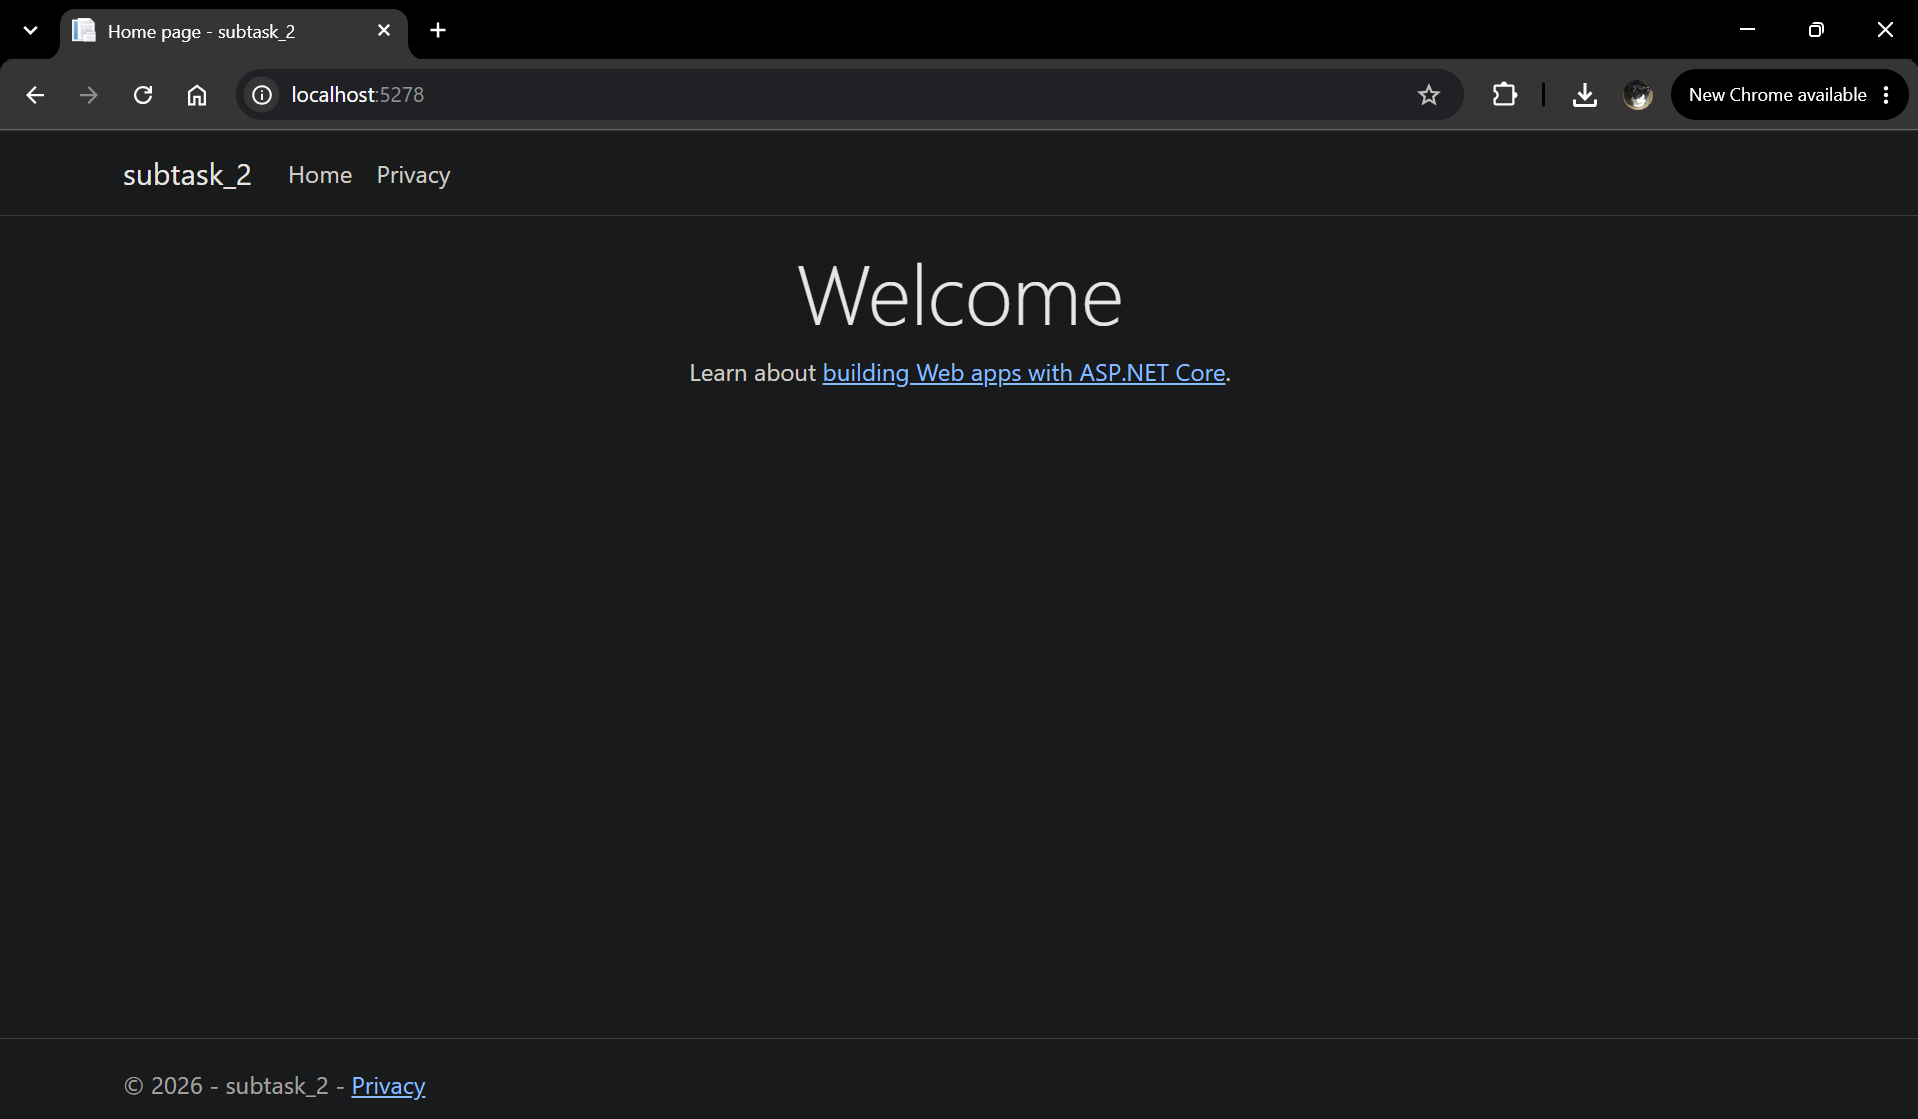
\includegraphics[scale=0.4]{images/2_test_local.jpg}
\vspace{-1em}
\caption{The application runs locally on port 5278.}
\end{figure}

Similar to Task 2.1, I created a new Web App Service instance using the Azure App Service extension. The new instance is named \texttt{swe40006-task-2-2}, hosted in the Australia East region, and using the .NET 8.0 runtime.

\begin{figure}[H]
\centering
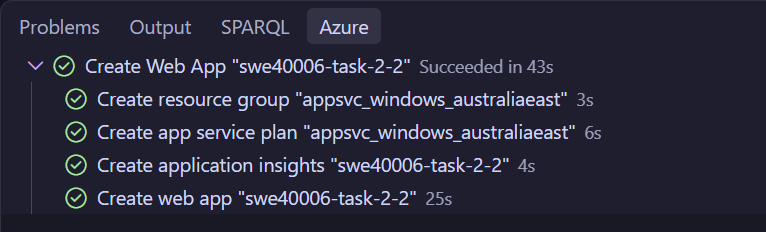
\includegraphics[scale=0.6]{images/2_create_web_app.jpg}
\vspace{-1em}
\caption{A new Web App Service instance is successfully created.}
\end{figure}

The application is then deployed into this new instance. It is hosted at \url{https://swe40006-task-2-2-f9emhph2gddzhker.australiaeast-01.azurewebsites.net/}.

\begin{figure}[H]
\centering
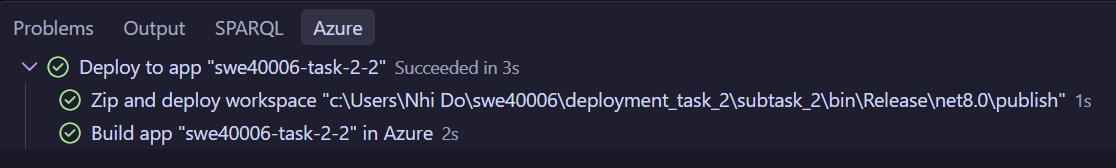
\includegraphics[scale=0.6]{images/2_deploy_app.jpg}
\vspace{-1em}
\caption{Successful deployment.}
\end{figure}

\begin{figure}[H]
\centering
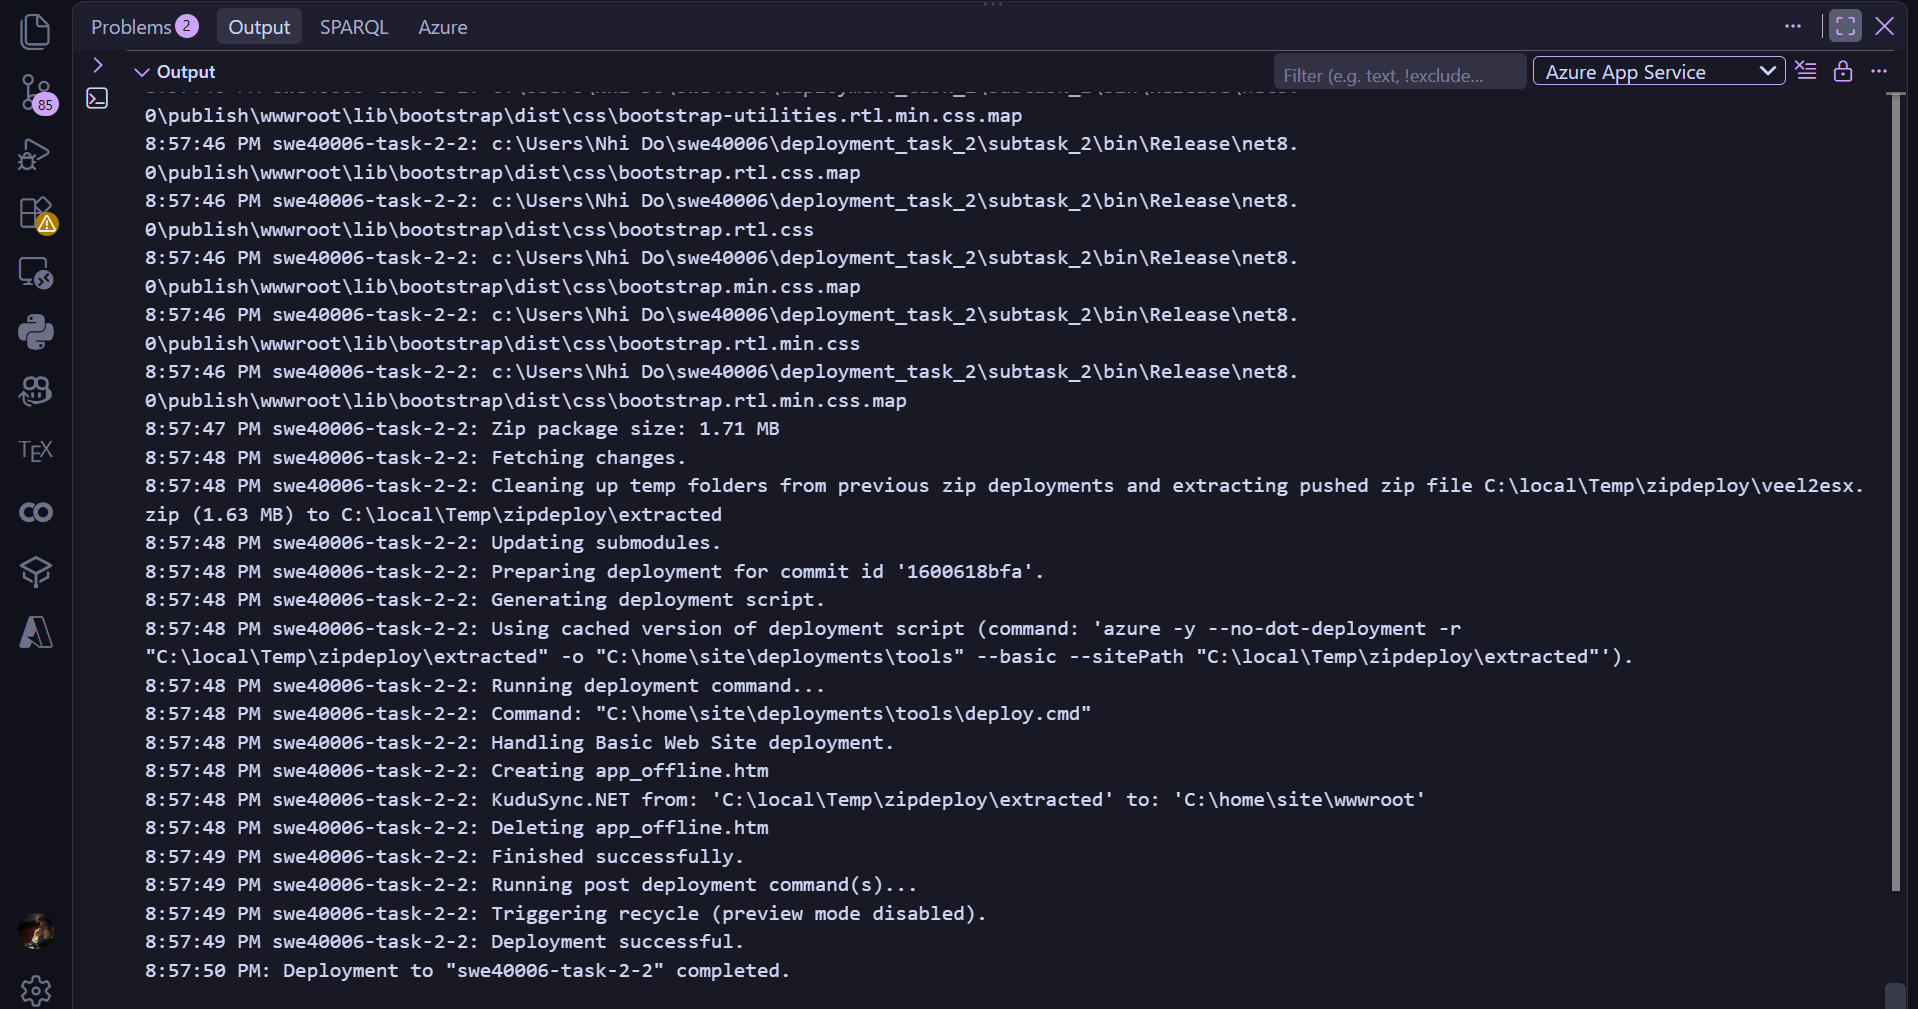
\includegraphics[scale=0.4]{images/2_build_output.jpg}
\vspace{-1em}
\caption{Logs showing that deployment was successful.}
\end{figure}

\begin{figure}[H]
\centering
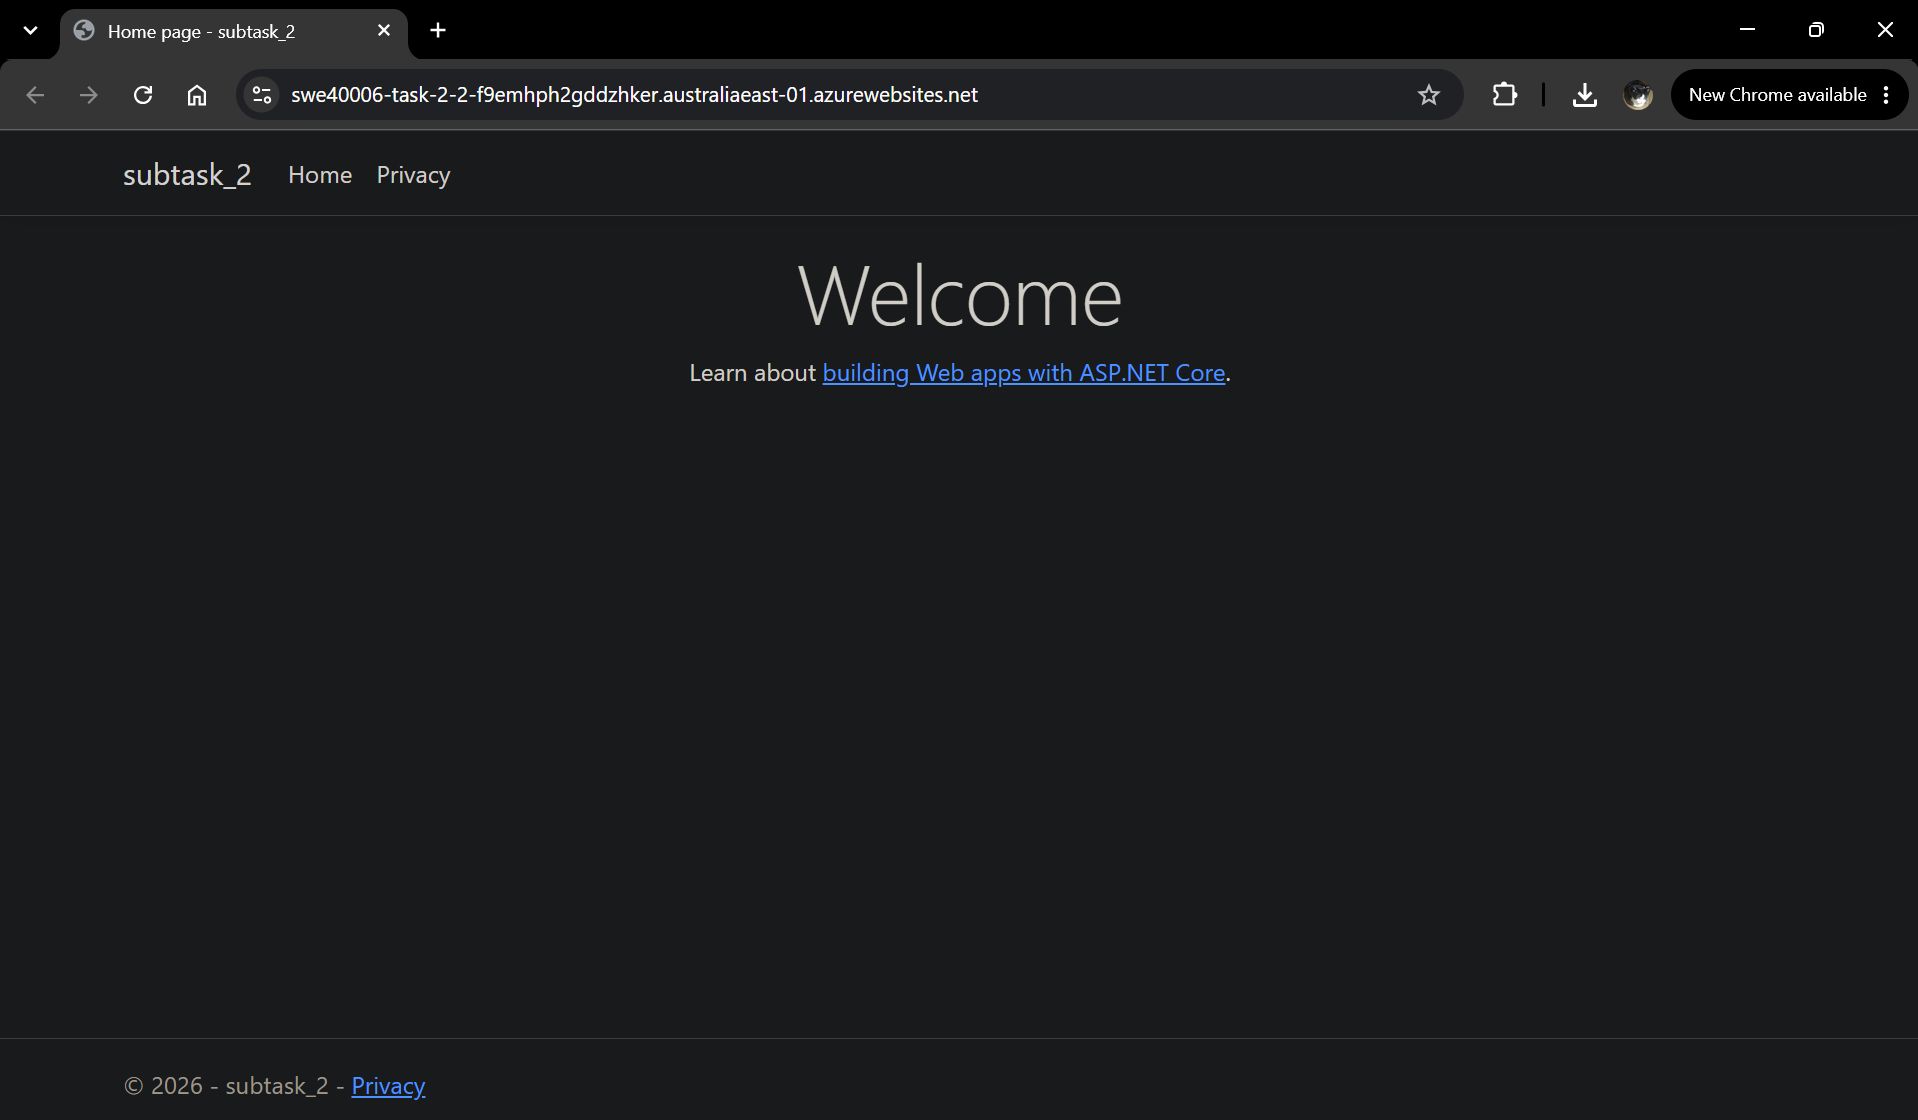
\includegraphics[scale=0.4]{images/2_live_site.jpg}
\vspace{-1em}
\caption{The web application up and running live.}
\end{figure}

Even though this App Service instance is running on a free tier, it is still best practice to manage cloud resources responsibly to avoid unintended charges. To demonstrate this, I stopped the instance using the Azure Portal.

\begin{figure}[H]
\centering
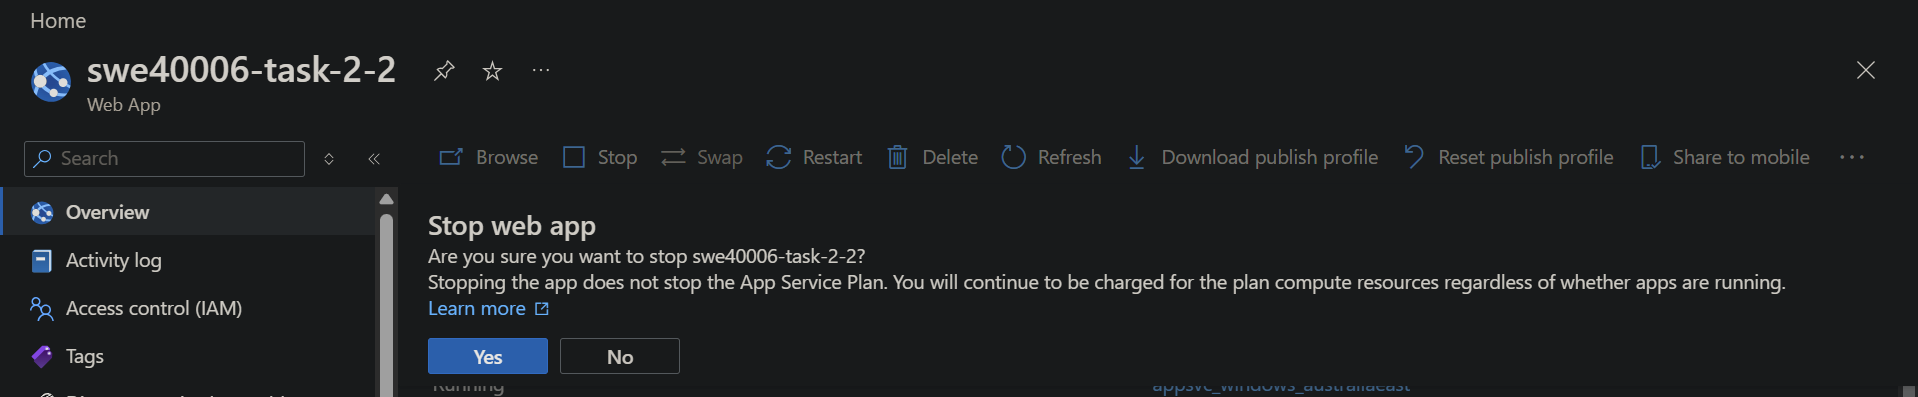
\includegraphics[scale=0.4]{images/2_stop_app.jpg}
\vspace{-1em}
\caption{Stopping the instance.}
\end{figure}

\begin{figure}[H]
\centering
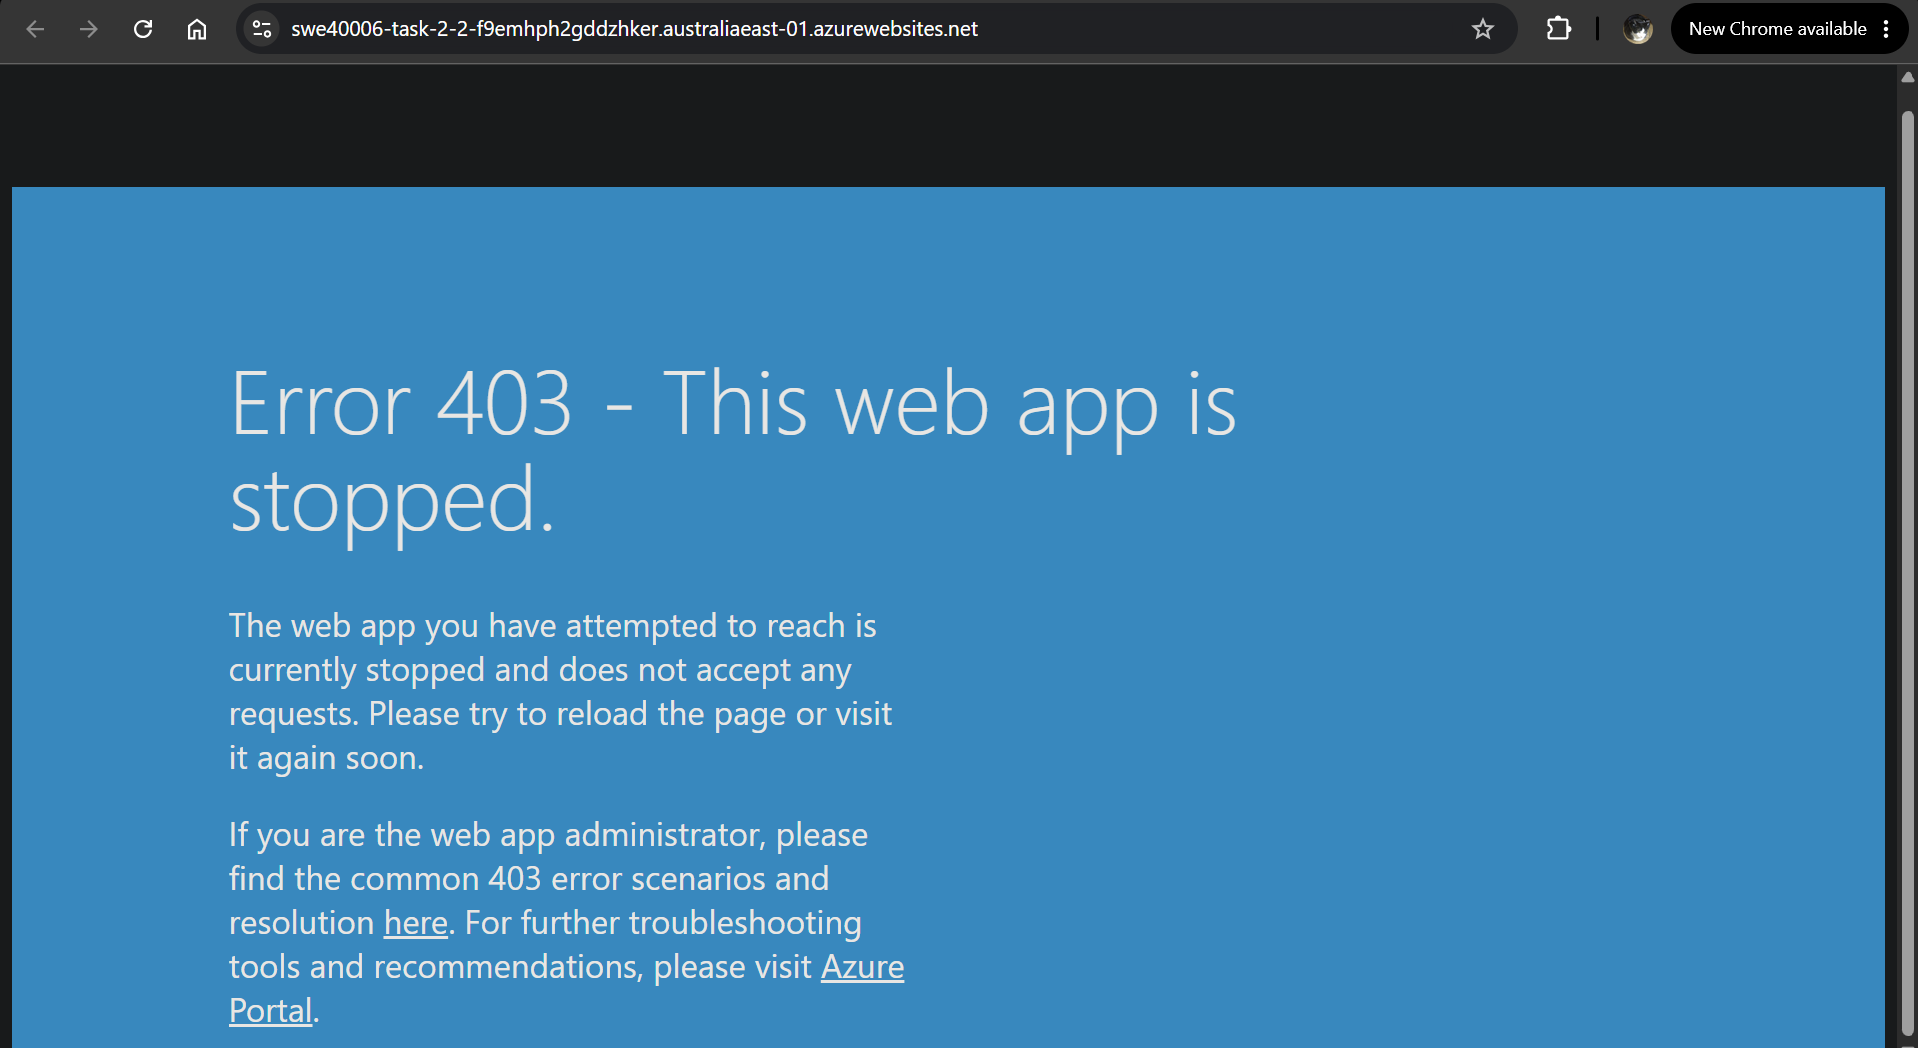
\includegraphics[scale=0.4]{images/2_stopped.jpg}
\vspace{-1em}
\caption{The web app has been stopped.}
\end{figure}

% References
% \printbibliography
\end{document}